%!TEX root = CS818_assessment.tex
The cluster analysis showed that the cluster associated with the highest obesity group was characterised by a family history of obesity, use of public transport, as well as frequent snacking and consumption of high calorie food. However, the cluster most strongly linked to normal weight also had strong associations with snacking and high calorie food, underscoring the high variability of diet's impact on individuals. It also suggests that whilst dietary habits play a significant role in obesity risk, their influence could be moderated in normal weight groups by other factors such as physical activity levels or a hereditary predisposition towards a certain weight. It could also be indicative of factors not well captured in the data such as variance in individuals' metabolic response to foods, which may allow some individuals to maintain a healthy weight despite a high caloric intake \cite{Piaggi2019}. Any cause-effect relationships therefore appear to be obscured by layers of behavioural, demographic and  genetic or hereditary interactions. These relationships were further interrogated with the decision-tree. 

Whilst the full decision-tree has too many branches to be easily interpretable, a look at the initial branches in figure \ref{fig:decision_tree}, which has a max branch depth of 3, highlights the model's most important features.

\begin{sidewaysfigure}
    \centering
    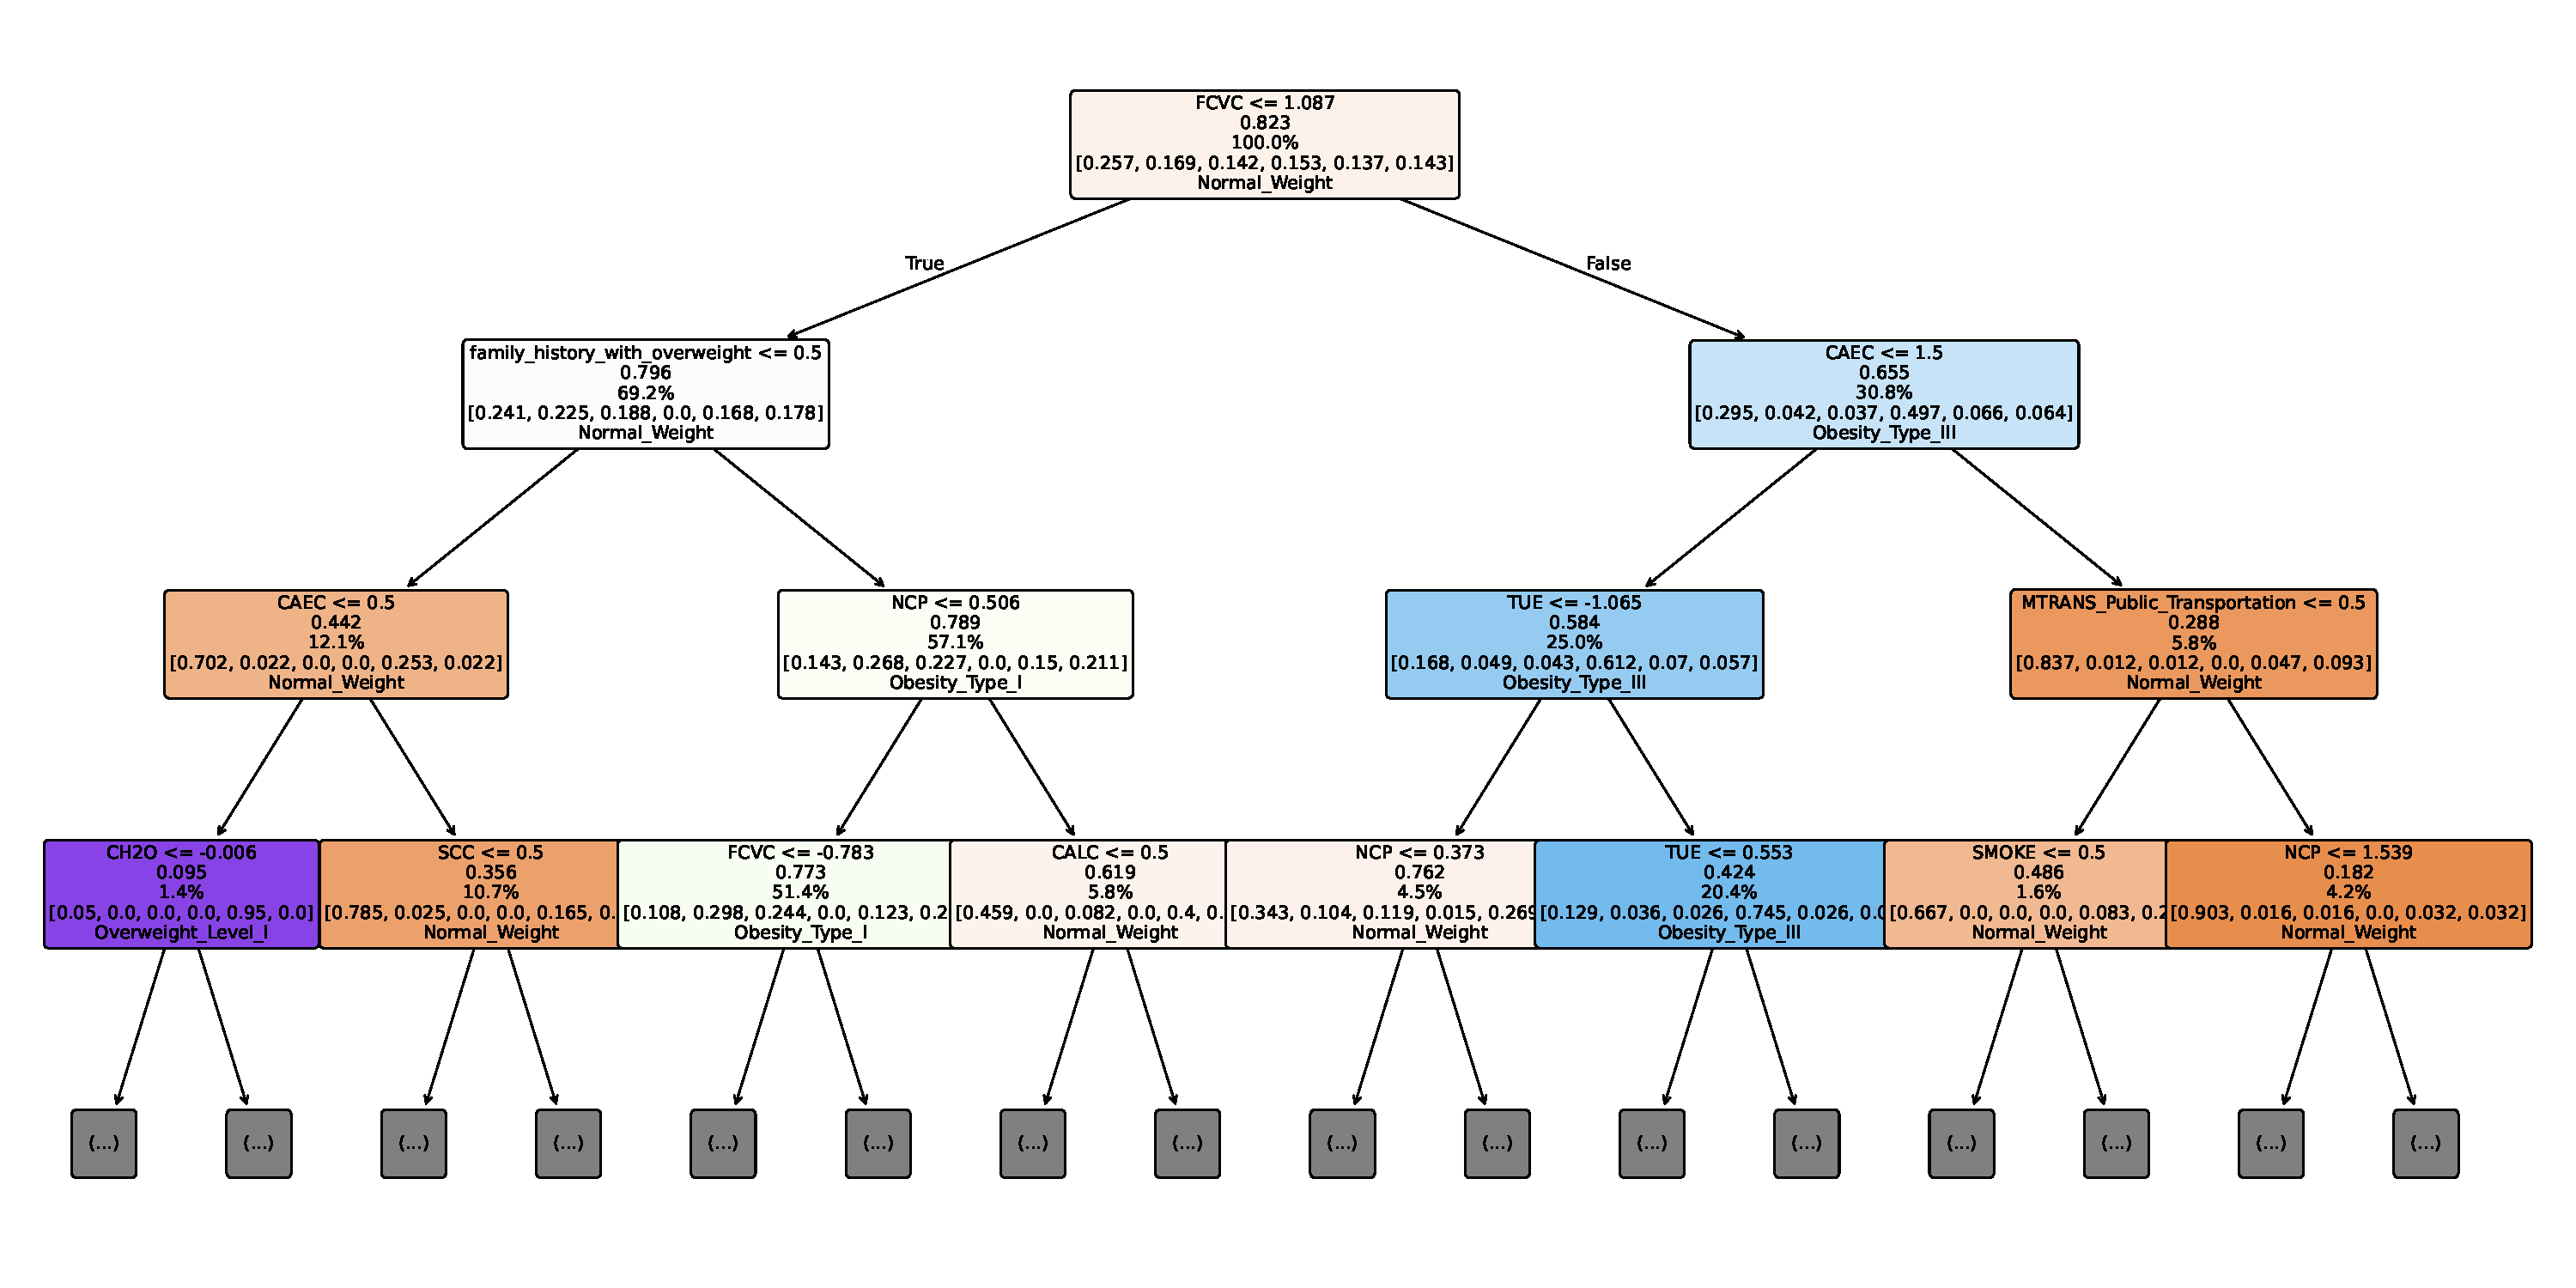
\includegraphics[width=\textwidth]{decision_tree.pdf} % Replace with your image
    \caption{Decision tree with a max depth of 3}
    \label{fig:decision_tree}
\end{sidewaysfigure}

This identifies some surprising relationships. For example, lower vegetable consumption appears to be generally associated with higher weight classes, however higher vegetable consumption together with more time spent on devices is linked to Obesity Type III, the group with the highest BMI. The relationship between FCVC and BMI was picked up in the initial exploratory analysis, but the decision-tree permits a deeper dive into the association, in particular by highlighting the influence of TUE. Whilst vegetable consumption may be predictive of obesity rates, the relationship here is not linear or omnidirectional. Instead, it is highly context dependent. The fact that high vegetable consumption appears to be generally linked to normal weight suggests it may have a protective effect in line with existing literature \cite{Nour2018}, however this impact may then be cancelled out by low physical activity. There may also be other factors not captured by the model that influence the high consumption amongst the highest BMI individuals. For example, people who are conscious of their weight may increase vegetable intake given public health messaging around the benefits, or it could reflect a 'social desirability bias'. This is where individuals are inclined to self-report socially desirable behaviours, which would lead them to over-report healthy behaviours and under-report unhealthy ones \cite{Hebert1995}. Seeking a better understanding of this relationship would be an interesting avenue for future research, given the extent to which it contradicts consensus in the literature. 
